% Quadrupole + Thomson scattering -> linear polarisation, redrawn from Hu & White (1997),
% New Astron. 2, 323, Fig. 1, on the slide palette (line thickness proportional to intensity).
% Compile: pdflatex -output-directory=.cache thomson_quadrupole.tex && pdftocairo -svg .cache/thomson_quadrupole.pdf thomson_quadrupole.svg
% Hot light comes down from the top, cold light in from the left; each ray carries its two
% polarisation directions (one in the plane, the diagonal one out of it). Scattering towards
% the lower right passes on the thick hot bar along x and the thin cold bar along y: the net
% polarisation lies along x, perpendicular to the hot direction.
\documentclass[tikz,border=4pt]{standalone}
\usepackage{tikz}
\usepackage[T1]{fontenc}
\usetikzlibrary{arrows.meta,decorations.markings}

\definecolor{ink}{HTML}{2E2E2E}
\definecolor{hot}{HTML}{C2560A}
\definecolor{cold}{HTML}{3B6FB6}
\definecolor{pcol}{HTML}{521463}

\tikzset{
  ray/.style={ink,line width=1.6pt,postaction={decorate},
    decoration={markings,mark=at position #1 with {\arrow{Stealth[length=4mm,width=3.4mm]}}}},
  hotbar/.style={hot,line width=3.6pt,line cap=round},
  coldbar/.style={cold,line width=1.3pt,line cap=round},
}

\begin{document}
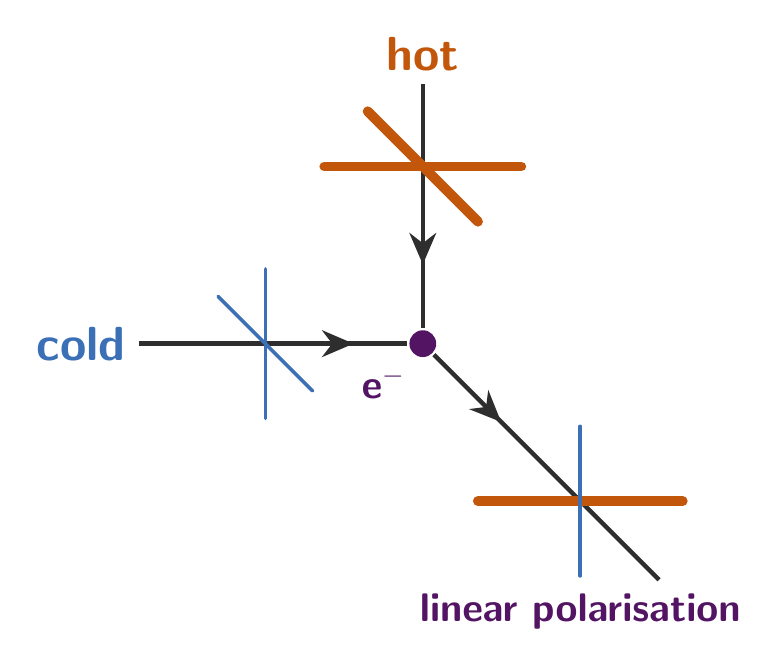
\begin{tikzpicture}[font=\sffamily]

% ---------------------------------------------------------------- rays
\draw[ray=0.74] (0,3.3) -- (0,0.2);        % hot, from above
\draw[ray=0.80] (-3.6,0) -- (-0.2,0);      % cold, from the left
\draw[ray=0.30] (0.14,-0.14) -- (3.0,-3.0); % scattered, towards us

% ---------------------------------------------------------------- polarisation crosses
% incoming hot: in-plane (x) and out-of-plane (diagonal)
\draw[hotbar] (-1.25,2.25) -- (1.25,2.25);
\draw[hotbar] (-0.7,2.95) -- (0.7,1.55);
% incoming cold: in-plane (y) and out-of-plane (diagonal)
\draw[coldbar] (-2.0,-0.95) -- (-2.0,0.95);
\draw[coldbar] (-2.6,0.6) -- (-1.4,-0.6);
% scattered: hot along x survives strong, cold along y weak
\draw[hotbar] (0.7,-2.0) -- (3.3,-2.0);
\draw[coldbar] (2.0,-1.05) -- (2.0,-2.95);

% ---------------------------------------------------------------- electron
\fill[pcol] (0,0) circle (0.17);
\node[pcol,font=\sffamily\bfseries\Large] at (-0.5,-0.5) {e$^-$};

% ---------------------------------------------------------------- labels
\node[hot,font=\sffamily\bfseries\LARGE,anchor=south] at (0,3.35) {hot};
\node[cold,font=\sffamily\bfseries\LARGE,anchor=east] at (-3.65,0) {cold};
\node[pcol,font=\sffamily\bfseries\Large,anchor=north,align=center] at (2.0,-3.05)
     {linear polarisation};

\end{tikzpicture}
\end{document}
